% -*- mode: fundamental -*-

% ****************************************************************

\chapter{The Fetch function: memory requests and responses}

\markboth{Ch \arabic{chapter}: Fetch, memory requests (DRAFT)}{\copyrightnotice}

\setcounter{page}{1}
% \renewcommand{\thepage}{\arabic{page}}
\renewcommand{\thepage}{\arabic{chapter}-\arabic{page}}

\label{ch_Fetch_function}

% ****************************************************************

\section{Introduction}

In this chapter we discuss the Fetch function of
Figure~\ref{Fig_Instr_Exec}, which we repeat here for convenience,
adding annotatinos on the arrows to show the \verb|struct| types they
communicate. All these \verb|struct| declarations can be found in the
file: \verb|src_Common/Inter_Stage.bsv|.
\begin{figure}[htbp]
  \centerline{\includegraphics[width=6in,angle=0]{ch030_RISCV_Design_Space/Figures/Fig_Instr_Exec_w_structs}}
  \caption{\label{Fig_Fetch_function_Simple_Instr_Exec}Simple interpretation of RISC-V instructions (same as Fig.~\ref{Fig_Instr_Exec}, with arrows annotated with {\tt struct} types)}
\end{figure}

The Fetch function \emph{per se} is fairly simple, even trivial.  Most
of our discussion is about the messages sent from the Fetch step to
memory (memory requests) and the messages returned from memory to the
Decode step (memory responses). The outputs of Read-PC-and-Fetch step
are:
\begin{tightlist}

 \item A \emph{memory request} to memory, to read an instruction.

 \item Some additional information passed on to the Decode step for subsequent use.

\end{tightlist}

// ****************************************************************

\section{RISC-V: the result-type of the Fetch function}

In Figure~\ref{Fig_Fetch_function_Simple_Instr_Exec}, the information
passed from the Fetch stage to the Decode stage is just the PC:

\begin{Verbatim}[frame=single, numbers=left]
typedef struct {
   Bit #(XLEN) pc;
} F_to_D
deriving (Bits, FShow);
\end{Verbatim}

\index{BSV!struct!Single-field structs}

It might seem like overkill to define a struct for just one field like
this, but it has the following advantages:

\begin{itemize}

  \item It becomes easy to add more fields later, should we need to do
    so.  In particular, for Fife we will need to add some
    branch-prediction information.  We may also wish to add temporary
    fields that aid in debugging.

  \item Stronger type-checking: each new struct type is distinct from
    all other types in a BSV program.  Thus, the type-checker will
    catch any error where we may inadvertantly pass some unrelated and
    irrelevant XLEN-wide value in place of an \verb|F_to_D| struct.

  \item There is \emph{no} runtime cost: an \verb|F_to_D| value
    occupies the same XLEN bits as the \verb|pc| field by itself.

\end{itemize}

\index{BSV!struct!Nested}

BSV structs can be nested.  The Fetch function's result is a nested
struct containing two structs, one being the memory-request to be sent
to memory, and the other being the information to be passed to the
Decode step:

\begin{Verbatim}[frame=single, numbers=left]
typedef struct {
   F_to_D   to_D;
   Mem_Req  mem_req;
} Result_F
deriving (Bits, FShow);
\end{Verbatim}

% ****************************************************************

\section{RISC-V: The Fetch Function}

\label{Sec_Fetch_function}

Finally, we can write the Fetch function, which is very simple, almost
trivial.  Its input is the current value of the program counter (PC),
and it returns a \verb|Result_F|.  The PC is used as the address from
which to read memory.

\begin{Verbatim}[frame=single, numbers=left]
function Result_F fn_F (Bit #(XLEN)  pc)
    Result_F y = ?;

    // Info to next stage
    y.to_D = F_to_D {pc: pc};

    // Request to IMem
    y.mem_req = Mem_Req {req_type: MEM_LOAD,
                         size:     MEM_4B,
                         addr:     pc,
                         data :    ?};        // don't-care value
      return y;
endfunction
\end{Verbatim}

% ================================================================

\subsection{BSV: Don't-care values} 

\index{BSV!{\tt ?}, the don't care value}
\index{BSV!AAAA\_AAAA, the default don't care value}

Since we are performing a LOAD, the value carried in the \verb|data|
field of the request is irrelevant.  Instead of placing some
particular but arbitrary value (such as ``0'') into that field, we use
BSV's ``\verb|?|'' notation for a don't-care value.

First, this conveys to the human reader that the value in this field
is irrelevant.

Second, it can result in more efficient circuitry.  If we had said
``0'', for example, the \emph{bsc} compiler would have had to create
circuitry that ensured that that field value was 0. By saying
``\verb|?|'', the \emph{bsc} compiler is allowed to omit all that
circuitry.

Third, in places where it does not result in additional hardware, the
\emph{bsc} compiler usually injects the specific value
\verb|'h_AAAA_AAAA| (of suitable bit-width).  While debugging,
observing such a value in some computation is often a clue that
something is wrong.

\vspace{2ex}

NOTE:
\fbox{\small
\begin{minipage}{5in}

Verilog and SystemVerilog have a concept of ``X'' values.  Each bit of
a register or wire carries an ``X'' value until it has been assigned a
specific binary value (0 or 1).  However, note that this is \emph{only
in simulation}, where the simulator can and does model 3-valued logic
(0, 1 and X) for each bit, and is able to propagate X values through
operators, registers, {\etc} Hardware only implements 2-valued
logic---every bit is either 0 or 1. Thus, this is an artefact that is
only useful during debugging in simulation.

\vspace{1ex}

BSV only has 2-valued logic; there is no concept of an ``X'' value.  A
BSV ``{\tt ?}'' expression has some specific, but potentially
unpredictable, binary value.

\end{minipage}}


% ****************************************************************
